\subsection{Overview and Research Question}
In this study we hoped to answer 2 research questions; 1) are there any benefits to adherence when patients are given medical prescriptions through audio in a native language that is not English, like isiXhosa, and secondly does the use of audio help patients recall and understand their prescriptions? This study is part of a larger study that looks at if there's any significant difference in adherence rates in giving patients their medical prescriptions in the local langauge and which mode (auido, text or through pictures) shows the most promise. To help answer all these questions, we set out to give patients their medical prescriptions in isiXhosa using audio recordings and monitor how they take their medication. Monitoring how they take their medication helps us answer questions around adherence. To answer questions around recall and comprehension we asked participants some open ended questions to test how easy they could remember the contents of their prescription and to see if they had indeed understood, with clarity, the contents and implications of the given prescriptions. It is worthnoting that this is not a clinical trial and as such we did not use actual patients but rather we asked isiXhosa speaking individuals to be part of the study. As this is not a clinical study, we used an app to simulate the process of a patient taking in medication, this is explained in more detail in Software Development section. The study was set out to start with a briefing session where we explained to the participants what the study is about and how we would go about conducting it. The patients/participants of the study then used the app for the next 5 days then returned after for a debrief session where we asked them questions to evaluate if they understood their prescriptions.

\subsection{Study Design}
\subsubsection{Participants}
We selected participants that were not only fluent in isiXhosa but were also comfortable in reading the language, reason being we did not want participants to favour one mode over the other (audio over reading) and introducing bias into the study. It was established that we were more likely to find such participants amongst the older isiXhosa speaking population as they are less frequently thwarted into scenarios requiring them to consume knowledge or interact in English, which is not the case with university students who learn primarily through English literature. And so we hoped to engage with the staff at the University of Cape Town (UCT) because we could easily access them but we were not able to secure the ethical clearance to do so in a timely fashion. Alas, we looked for participants from outside UCT, we talked to people that worked in shops, fuel refill stations, churchgoers after service and security guards. After talking to more than 25 people, we were able to successfully convince at least 12 people to be part of the study. Because of the nature of their work, we could not find a common time when everyone was free, and so we had to hold individual sessions, some would come in twos but mostly each participant came to the debrief session alone. To make sure that we give all participants the same information during the breifing session, we wrote a script of how the session would be conducted. Thus, the only difference in the information participants got would be through questions that each posed during the briefing session. These participants were split into two groups; control and the ones that received the audio treatment. This ended up being 2 groups of 5 as 2 participants did not return for the debrief session.

\subsection{Prescription}
In coming up with the prescriptions, we used the findings of a paper published by Berry et al \cite{Berry} where by the researchers ran 3 studies to determine what should the contents of a prescription include. In that study, Berry et al concluded that for a prescription to be considered sufficient, it should at least address 3 issues. Firstly, what is the medication for, secondly what are the side effects and finally what are the lifestyle changes that the patient should implement in order for him/her to experience the full benefits of the medication.
We fabricated a prescription for back pain. We intentionally chose not to use a known prescription because we did not want any participant recognizing the prescription and thus coming in with prior knowledge into the study which could skew our results. We wanted each participant to receive this relatively new information and be evaluated in the same manner. Both groups were given the same prescription, but in different formats. The control group was given the prescription through a pillcard that resembled the pillcards being given to patients in South African hospitals. It is worth noting that these are often in English and as such we gave our control group pillcards containing their prescriptions written in English. For the audio group, the prescription was recorded in isiXhosa the uploaded on a cloud database, firebase\footnote{Firebase is google's realtime database engine for mobile apps - https://firebase.google.com/}. In accordance with the recommendation of Davis et al, we made tried to make the recording as clear and concise as possible. keeping the record under 2 mins without leaving out any crucial information. We went a step further to record the 3 different sections that Berry et al mentioned in his paper separately; thus there was a recording explaining what the medication is for and how to administer it, there was a recording on what are the possible side effects and there weas a recrding explaining the lifestyle changes.

\subsubsection{Software Development}
As we have previously mentioned this is not a clinical study, therefore meaning that we did not give patients any real medication. To help us monitor adherence rates, we designed a mobile app that simulates the process of taking in medication. The idea was that patients would push a button and that would represent them taking their medication. For instance, if a patient is to take 3 pills at night, we would expect the participant to push the button 3 times. Additionally, we added a button that displays a screen where the patient can then listen to their prescriptions, but that was a button only available to the audio group as the control group had their prescription through their pillcard. The two screens for audio are shown below.

\begin{figure}
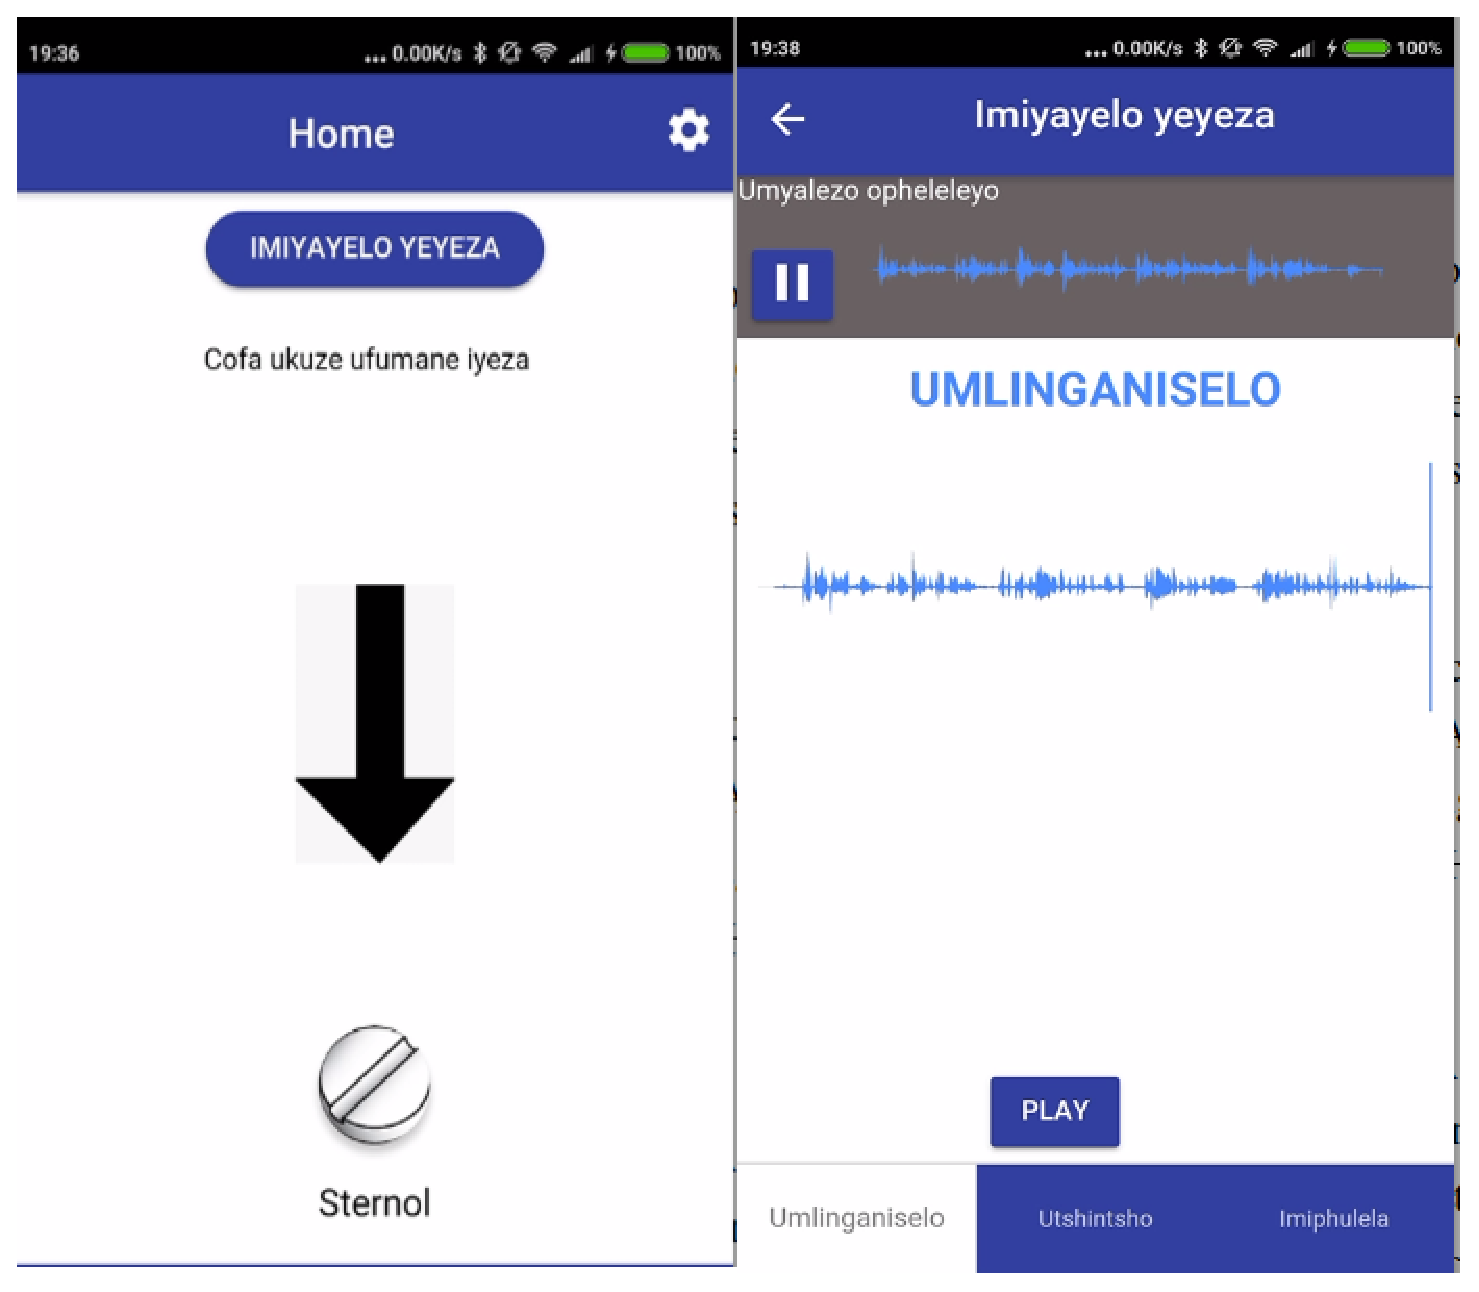
\includegraphics[width=\linewidth, height=200pt]{mobileapp}
\caption{A sceenshot of the home screen and the listening screen}
\end{figure}

To develop this app we used the ionic\footnote{Ionic 4 - ionicframework.com}, which allowed for us to develop a hybrid app that can be used across multiple platforms, or so we had hoped. Eventually it turned out that the version of ionic, version 4, we were using is not compatible with windows mobile phones and
due to financial constraints we could not compile an iOS\footnote{The operating system running on Apple phones, https://www.apple.com/za/ios/ios-10/} compatible version of the software\footnote{To write Apple apps one must have an apple console, to register an apple console one must register through their Apple Development Programme of which has a registration fee of 99USD}. Alas we had an android app, fortunately most of our participants had android phones. Ionic uses a webview\footnote{cordova - cordova.apache.org} as a wrapper to display all its components. It therefore allows developers to write mobile apps using web development tools such as AngularJS, HTML5 and SCSS to name a few, also one can use other javascript plugins that they deem necessary, as one does in web development. In fact, we did also use a number of opensource javascript plugins, like angularfire2\footnote{A plugin to connect your ionic v4 app to your firebase database and cloud storage - we used version 4.0.0-rc.2}.

For our database, we setup 13 separate users, 6 users for each group and a test user used during development. Firebase is a NoSQL database meaning all users were essentially a key-value pair where the user is the key and the value represents a collection of attributes for each user. These attributes helped us keep track of which users were already assigned and which prescription they were meant to on.

Participants were given the app through an app called ShareIt. After installing, the participants had to be assigned to the already populated user list in the database, at this time it did not matter much which user they were set to because there is only one prescription but since this is part of an ongoing study we might decide to have other users listen to different medical prescriptions, therefore needing the prescription variable to be dynamic. When the user is set, the prescription is read of that user profile and the corresponding audio files were downloaded from our firebase storage server. These files will sit locally on the phone, henceforth allowing the participant to play back the recordings without incuring any data costs.

Lastly the app is recording the time and date when a user presses on the button to take the medication.
